\documentclass[11pt,a4paper]{article}
\usepackage[utf8]{inputenc}
\usepackage[T1]{fontenc}
\usepackage[ngerman]{babel}
\usepackage{geometry}
\geometry{a4paper, left=2.5cm, right=2.5cm, top=2.5cm, bottom=2.5cm}
\usepackage[hidelinks]{hyperref}
\usepackage{enumitem}
\usepackage{graphicx}
\usepackage{xcolor}
\usepackage{float}

% Colors for User Stories
\definecolor{usgray}{RGB}{240, 244, 248}
\definecolor{usblue}{RGB}{41, 128, 185}

\title{\textbf{Anforderungsspezifikation \& Sprint Backlog} \\ \large Entwicklung \& Evaluation eines Konzepts zur automatisierten Transformation unstrukturierter Produktdaten mittels großer Sprachmodelle}
\author{Fabian Lohoff (Matrikelnummer: 9051803)}
\date{\today}

\begin{document}

\maketitle

\begin{abstract}
    \noindent Dieses Dokument fasst die funktionalen, nicht-funktionalen und technischen Anforderungen für den Projektteil der Bachelorarbeit zusammen. Gegenüber der ursprünglichen Fassung berücksichtigt diese Version zusätzlich das lokale MongoDB-Datenmodell mit Batch-Verarbeitung, persistierten Transformationszuständen, Schema-Validierung, Normalisierung, Produkt-Matching, API-Export und Bewertungsexport. Die Anforderungen bilden die Grundlage für die Sprintplanung und die Implementierung der Softwarearchitektur.
\end{abstract}

\tableofcontents
\newpage

\section{Einleitung und Systemkontext}

Das zu entwickelnde System dient der automatisierten Transformation unstrukturierter Produktdaten in ein strukturiertes, API-konformes Ziel-JSON. Die Transformation erfolgt nicht mehr ausschließlich als flüchtige Pipeline, sondern wird über eine lokale MongoDB-Zwischendatenbank nachvollziehbar persistiert. Dadurch können Eingabedaten, Zwischenergebnisse, LLM-Ausgaben, Normalisierungsergebnisse, Matching-Entscheidungen, Exportresultate und Evaluationsmetriken reproduzierbar gespeichert und ausgewertet werden.

Das in Abbildung~\ref{fig:kontextdiagramm} dargestellte Kontextdiagramm veranschaulicht die informationstechnische Einbettung und den Datenfluss des zu entwickelnden Transformations-Systems:

\begin{figure}[htbp]
    \centering
    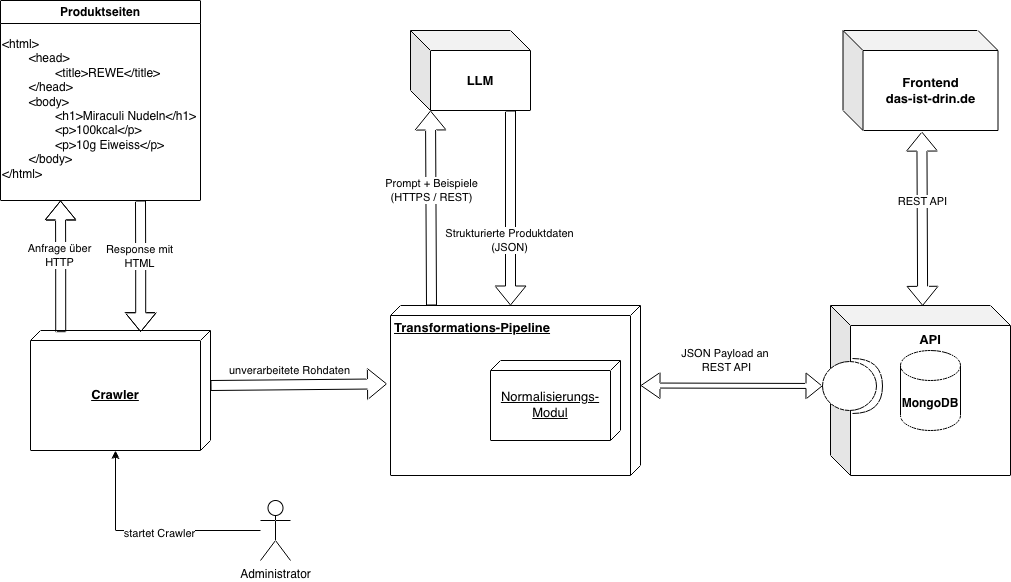
\includegraphics[width=0.95\textwidth]{ContextDiagram.png}
    \caption{Systemkontext der Transformations-Pipeline mit integriertem Normalisierungs-Modul}
    \label{fig:kontextdiagramm}
\end{figure}

Der Gesamtprozess gliedert sich in folgende Kernkomponenten:

\begin{enumerate}
    \item \textbf{Input \& Vorverarbeitung:} Produktdaten können über eine REST-Schnittstelle oder einen Datei-Input in das System gelangen. Die Eingangsdaten enthalten mindestens eine Produkt-URL, den Shop bzw. die Quelle und optional HTML-Rohtext, externe IDs sowie Bildinformationen.
    
    \item \textbf{Batch-Verarbeitung:} Eingehende Transformationsaufträge werden in einem \texttt{BatchRequest} zusammengefasst. Jeder einzelne Produktdatensatz wird als \texttt{TransformationRequest} modelliert und besitzt einen eigenen Verarbeitungsstatus. Dadurch können Batchläufe kontrolliert, wieder aufgenommen und ausgewertet werden.
    
    \item \textbf{Lokale MongoDB-Zwischendatenbank:} Die Pipeline speichert alle relevanten Daten und Zwischenergebnisse in einer lokalen MongoDB. Diese lokale Datenbank dient ausschließlich der Entwicklung, Nachvollziehbarkeit, Evaluation und Zwischenspeicherung. Sie ersetzt nicht die produktive Datenbank und stellt keine direkte Schreibverbindung zum Produktivsystem dar.
    
    \item \textbf{LLM-Schnittstelle (Gemini API):} Die in Python implementierte Transformations-Pipeline kommuniziert via HTTPS/REST mit der Gemini API. Über strukturierte Prompts wird das LLM angewiesen, die unstrukturierten Daten semantisch zu interpretieren und als strukturiertes JSON-Objekt zurückzugeben.
    
    \item \textbf{Schema-Validierung:} Die LLM-Ausgabe wird gegen ein vordefiniertes internes JSON-Schema geprüft. Validierungsfehler werden im jeweiligen \texttt{TransformationRequest} gespeichert, sodass Schema-Konformität quantitativ ausgewertet werden kann.
    
    \item \textbf{Normalisierungs-Modul:} Nach der Extraktion werden Mengen-, Größen- und Nährwertangaben deterministisch normalisiert. Gewichte werden in Gramm und Flüssigkeitsmengen in Milliliter überführt. Die normalisierten Daten werden getrennt von der rohen LLM-Ausgabe gespeichert.
    
    \item \textbf{Regelbasierter Vergleichsansatz:} Zusätzlich wird ein regelbasierter Ansatz zur Extraktion von Verpackungsgrößen implementiert. Dieser dient als deterministische Baseline für den wissenschaftlichen Vergleich mit dem LLM-basierten Ansatz.
    
    \item \textbf{Produkt-Matching \& API-Anbindung:} Vor der finalen Datenübergabe erfolgt ein Dublettenabgleich mit bereits bekannten Produkten. Anschließend wird aus den lokal gespeicherten und normalisierten Daten ein Ziel-JSON erzeugt und an die bereitgestellte REST- oder GraphQL-API übertragen. Die finale Persistierung im Produktivsystem erfolgt ausschließlich über diese API.
    
    \item \textbf{Evaluation \& Bewertungsexport:} Die erzeugten Daten werden anhand definierter Metriken bewertet. Ergebnisse wie Schema-Compliance, Exact Match Rate, Precision, Recall, F1-Score, Laufzeit und Kosten können pro \texttt{TransformationRequest} und aggregiert pro \texttt{BatchRequest} exportiert werden.
\end{enumerate}

\subsection{Datenmodell}

Das lokale Datenmodell unterscheidet zwischen Collections, eingebetteten Objekten und Enums. Collections sind eigenständig persistierte MongoDB-Dokumente, während eingebettete Objekte innerhalb eines übergeordneten Dokuments gespeichert werden.

\begin{figure}[H]
    \centering
    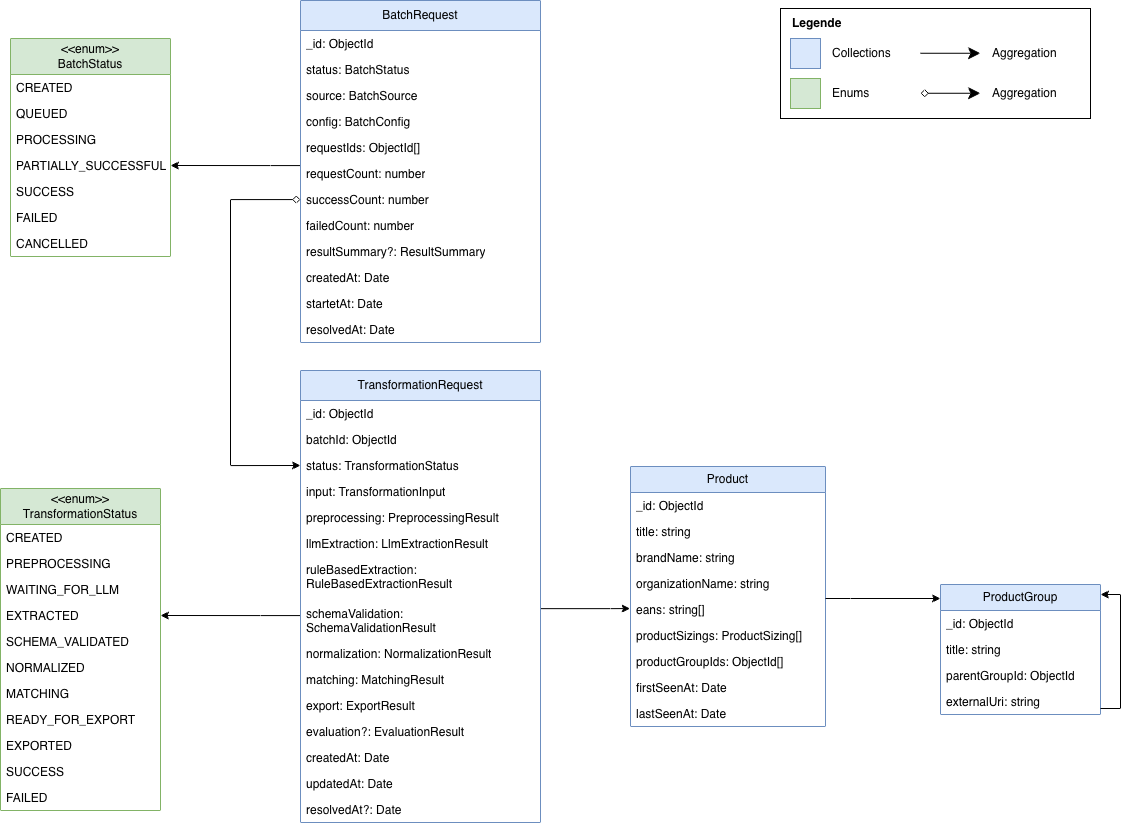
\includegraphics[width=0.95\textwidth]{DB_Short.png}
    \caption{Vereinfachtes lokales Datenmodell mit BatchRequest, TransformationRequest, Product und ProductGroup}
    \label{fig:db-short}
\end{figure}

\begin{figure}[H]
    \centering
    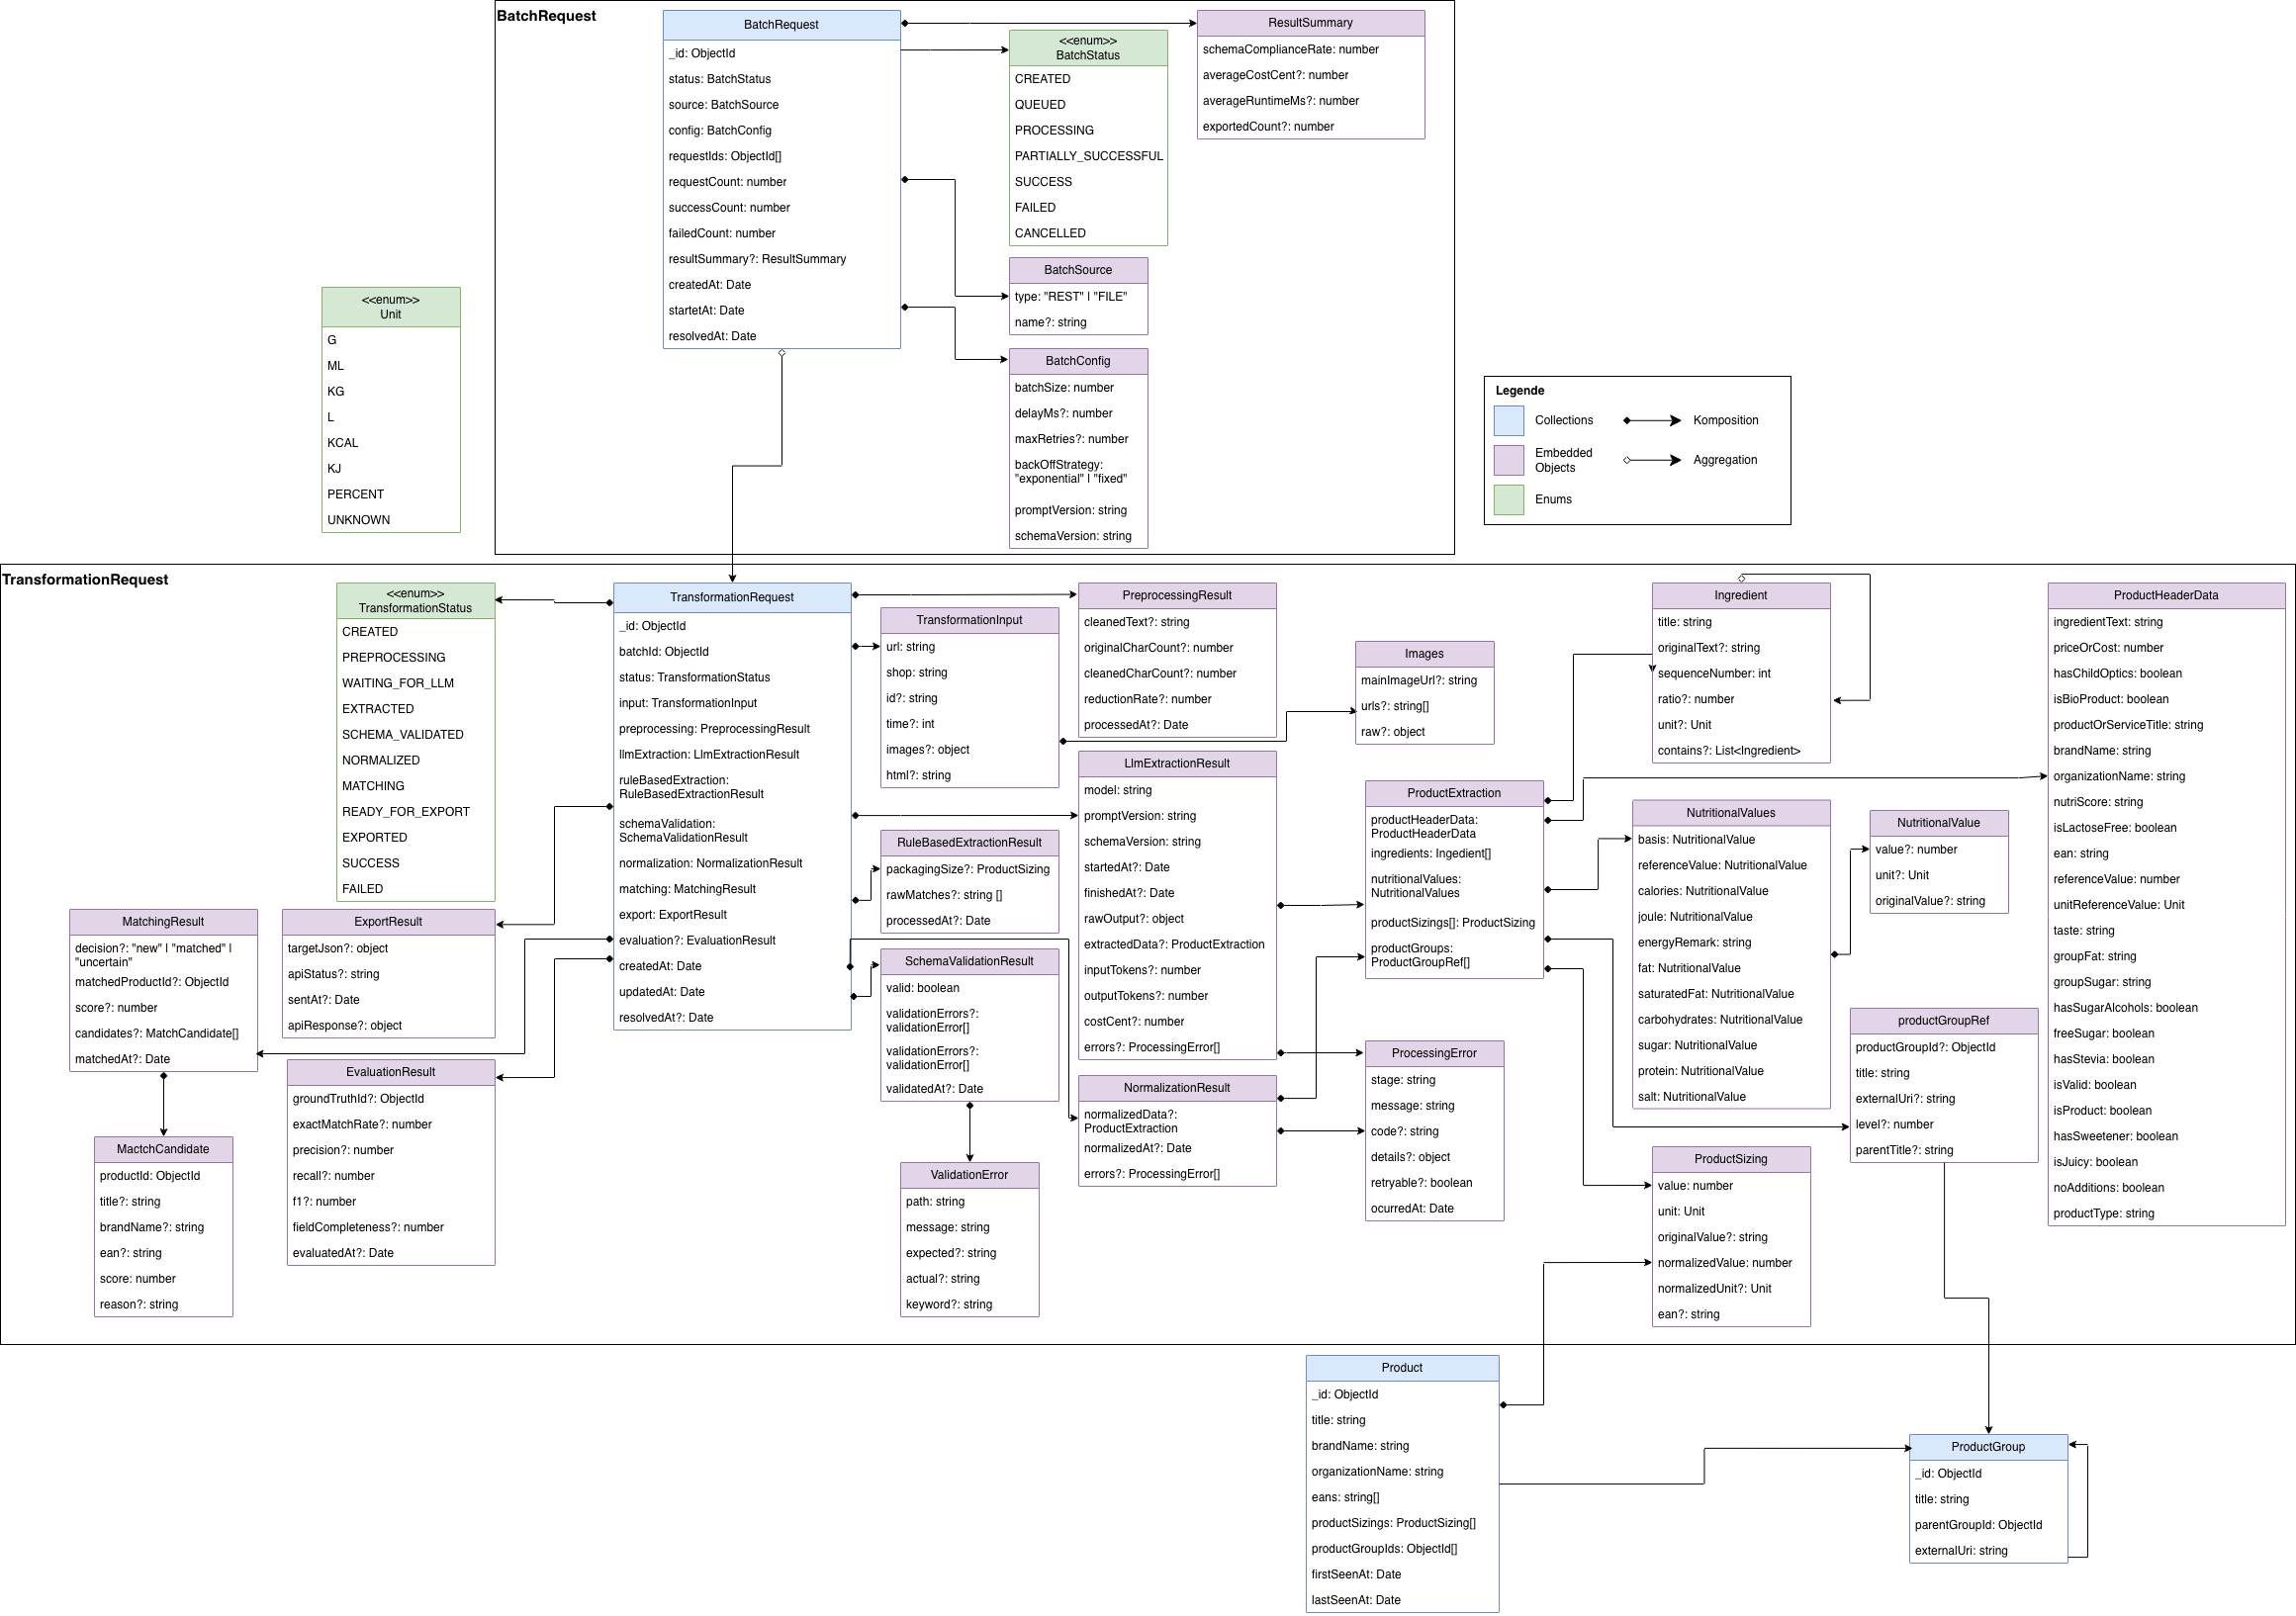
\includegraphics[width=0.95\textwidth]{DB_Long.png}
    \caption{Erweitertes lokales Datenmodell mit eingebetteten Transformations-, Extraktions-, Validierungs-, Normalisierungs- und Evaluationsobjekten}
    \label{fig:db-long}
\end{figure}

Die zentrale Arbeits-Collection ist \texttt{TransformationRequest}. Sie bildet den vollständigen Lebenszyklus eines einzelnen Produkts ab: Eingabe, Vorverarbeitung, LLM-Extraktion, regelbasierte Extraktion, Schema-Validierung, Normalisierung, Matching, Export und Evaluation. Der \texttt{BatchRequest} dient als organisatorische Klammer für mehrere Transformationsaufträge und speichert aggregierte Ergebniswerte.

\newpage
\section{Funktionale Anforderungen (FA)}

\subsection{Phase 1: Input, Vorverarbeitung \& Batch-Verwaltung}

\begin{itemize}[leftmargin=*]
    \item \textbf{FA 1.1 (Mehrere Eingangsquellen):} Das System muss Transformationsaufträge sowohl über eine REST-Schnittstelle als auch über einen Datei-Input entgegennehmen können. Die Quelle eines Batchlaufs muss im Objekt \texttt{BatchSource} dokumentiert werden.
    
    \item \textbf{FA 1.2 (HTML-Cleaning):} Das System muss HTML-Rohtexte von im Kontext irrelevantem Ballast wie Scripts, Styles, Footer- und Navigationselementen befreien, um Token-Kosten zu sparen und das Rauschen für das LLM zu minimieren.
    
    \item \textbf{FA 1.3 (Batch-Erzeugung):} Das System muss mehrere eingehende Transformationsaufträge zu einem \texttt{BatchRequest} zusammenfassen können. Jeder einzelne Auftrag muss als \texttt{TransformationRequest} mit eigener ID, eigenem Status und eigener Verarbeitungshistorie gespeichert werden.
    
    \item \textbf{FA 1.4 (Konfigurierbare Batch-Verarbeitung):} Das System muss Batch-Größe, Delay zwischen API-Aufrufen, maximale Wiederholungsversuche und Backoff-Strategie konfigurierbar machen. Diese Parameter müssen im Objekt \texttt{BatchConfig} dokumentiert werden.
    
    \item \textbf{FA 1.5 (Persistenz von Zwischenständen):} Das System muss alle relevanten Zwischenstände eines Transformationsauftrags in der lokalen MongoDB persistieren. Dazu gehören Inputdaten, bereinigter Text, LLM-Ausgabe, Validierungsergebnisse, Normalisierungsergebnisse, Matching-Ergebnisse, Exportstatus und Evaluationswerte.
    
    \item \textbf{FA 1.6 (Statusverwaltung):} Das System muss für Batch- und Einzelaufträge definierte Statuswerte verwenden. Ein \texttt{BatchRequest} verwendet den \texttt{BatchStatus}, ein \texttt{TransformationRequest} den \texttt{TransformationStatus}.
\end{itemize}

\subsection{Phase 2: Extraktion \& LLM-Steuerung}

\begin{itemize}[leftmargin=*]
    \item \textbf{FA 2.1 (JSON-Contract):} Das System muss das LLM über strukturierte Prompts bzw. Structured Outputs dazu anweisen, ausschließlich ein valides, vordefiniertes JSON-Format zurückzugeben.
    
    \item \textbf{FA 2.2 (Produktdatenextraktion):} Das System muss aus unstrukturierten Produktdaten ein \texttt{ProductExtraction}-Objekt erzeugen. Dieses umfasst mindestens \texttt{ProductHeaderData}, \texttt{Ingredient[]}, \texttt{NutritionalValues}, \texttt{ProductSizing[]} und \texttt{ProductGroupRef[]}.
    
    \item \textbf{FA 2.3 (Hierarchische Extraktion):} Das System muss geschachtelte Produktstrukturen, insbesondere Zutatenlisten mit Unterzutaten, in strukturierte Objekte überführen. Verschachtelte Zutaten müssen über \texttt{Ingredient.contains} abbildbar sein.
    
    \item \textbf{FA 2.4 (Speicherung der LLM-Metadaten):} Das System muss technische Metadaten des LLM-Aufrufs speichern. Dazu gehören Modellname, Prompt-Version, Schema-Version, Start- und Endzeitpunkt, Rohantwort, Token-Anzahlen, geschätzte Kosten und mögliche Fehler.
    
    \item \textbf{FA 2.5 (Schema-Validierung):} Das System muss die extrahierten Daten gegen ein definiertes Schema prüfen. Das Ergebnis wird als \texttt{SchemaValidationResult} gespeichert und enthält einen booleschen Validitätswert sowie optionale \texttt{ValidationError}-Einträge.
\end{itemize}

\subsection{Phase 3: Normalisierung \& regelbasierter Vergleich}

\begin{itemize}[leftmargin=*]
    \item \textbf{FA 3.1 (Einheiten-Normalisierung):} Nach der Überführung in strukturierte Daten müssen alle extrahierten Größen- und Mengenangaben in standardisierte Basiseinheiten transformiert werden. Gewichte werden in Gramm und Flüssigkeitsmengen in Milliliter normalisiert.
    
    \item \textbf{FA 3.2 (Typisierte Mengenwerte):} Mengen-, Verpackungs- und Nährwertangaben müssen intern als numerische Werte mit Einheit gespeichert werden. Originalwerte dürfen zusätzlich als String erhalten bleiben, um die Nachvollziehbarkeit der Extraktion zu gewährleisten.
    
    \item \textbf{FA 3.3 (Normalisierungsergebnis):} Das Ergebnis der Normalisierung muss als \texttt{NormalizationResult} im jeweiligen \texttt{TransformationRequest} gespeichert werden. Dabei muss zwischen roher LLM-Extraktion und normalisierten Produktdaten unterschieden werden.
    
    \item \textbf{FA 3.4 (Regelbasierte Verpackungsgrößen-Extraktion):} Das System muss einen regelbasierten Ansatz zur Extraktion von Verpackungsgrößen implementieren. Dieser kann auf regulären Ausdrücken oder heuristischen Regeln basieren.
    
    \item \textbf{FA 3.5 (Baseline-Vergleich):} Die Ergebnisse der regelbasierten Verpackungsgrößen-Extraktion müssen getrennt von der LLM-Extraktion gespeichert werden, um einen direkten Vergleich von Exact Match, Precision, Recall und F1-Score zu ermöglichen.
    
    \item \textbf{FA 3.6 (Fehlerbehandlung):} Fehler aus Normalisierung, LLM-Aufruf, Validierung oder Export müssen als \texttt{ProcessingError} bzw. \texttt{ValidationError} dokumentiert werden.
\end{itemize}

\subsection{Phase 4: Produkt-Matching, lokale Produktdaten \& API-Übertragung}

\begin{itemize}[leftmargin=*]
    \item \textbf{FA 4.1 (Lokale Produktdatenbank):} Das System muss eine lokale MongoDB verwenden, in der kanonische Produkte als \texttt{Product} und Produktgruppen als \texttt{ProductGroup} gespeichert werden können.
    
    \item \textbf{FA 4.2 (Produkt-Matching):} Nach Extraktion und Normalisierung müssen Produktdaten gegen lokal bekannte Produkte abgeglichen werden. Das Matching-Ergebnis wird als \texttt{MatchingResult} gespeichert.
    
    \item \textbf{FA 4.3 (Matching-Kandidaten):} Das System muss mehrere mögliche Matching-Kandidaten speichern können. Jeder Kandidat wird als \texttt{MatchCandidate} mit Produkt-ID, optionalem Titel, Marke, EAN, Score und Begründung gespeichert.
    
    \item \textbf{FA 4.4 (Dublettenentscheidung):} Das System muss unterscheiden können, ob ein Produkt neu ist, einem bestehenden Produkt zugeordnet werden kann oder eine unsichere Entscheidung vorliegt.
    
    \item \textbf{FA 4.5 (Ziel-JSON-Erzeugung):} Aus den normalisierten lokalen Daten muss ein Ziel-JSON erzeugt werden, das dem erwarteten Format der Ziel-API entspricht.
    
    \item \textbf{FA 4.6 (API-Datenübergabe):} Das erzeugte Ziel-JSON darf nicht direkt in die produktive MongoDB geschrieben werden. Die Übergabe erfolgt ausschließlich über eine bereitgestellte REST- oder GraphQL-API.
    
    \item \textbf{FA 4.7 (Exportstatus):} Das Ergebnis der API-Übergabe muss als \texttt{ExportResult} gespeichert werden. Dazu gehören Ziel-JSON, API-Status, Sendezeitpunkt und API-Antwort.
\end{itemize}

\subsection{Phase 5: Evaluation \& Bewertungsexport}

\begin{itemize}[leftmargin=*]
    \item \textbf{FA 5.1 (Einzelbewertung):} Das System muss für jeden \texttt{TransformationRequest} Evaluationswerte speichern können. Dazu gehören Ground-Truth-Referenz, Exact Match Rate, Precision, Recall, F1-Score und Feldvollständigkeit.
    
    \item \textbf{FA 5.2 (Batch-Zusammenfassung):} Das System muss aggregierte Ergebniswerte pro Batch speichern. Dazu gehören Schema-Compliance-Rate, durchschnittliche Kosten, durchschnittliche Laufzeit und Anzahl exportierter Produkte.
    
    \item \textbf{FA 5.3 (Bewertungsexport):} Das System muss Evaluations- und Batch-Ergebnisse in einem maschinenlesbaren Format exportieren können, z.\,B. als JSON oder CSV.
    
    \item \textbf{FA 5.4 (Nachvollziehbarkeit):} Für jede Bewertung muss nachvollziehbar sein, auf welcher Eingabe, welchem Prompt, welchem Schema und welchem Normalisierungsergebnis sie basiert.
\end{itemize}

\section{Nicht-Funktionale Anforderungen (NFR)}

\begin{itemize}[leftmargin=*]
    \item \textbf{NFR 1 (Robustheit / Schema-Compliance):} Mindestens 95\,\% der vom System aufbereiteten JSON-Objekte müssen ohne strukturellen Fehler direkt vom Schema der Ziel-API akzeptiert werden.
    
    \item \textbf{NFR 2 (Kostenkontrolle \& Wirtschaftlichkeit):} Die durchschnittlichen API-Kosten der Gemini-Aufrufe pro transformierter Produktseite dürfen einen Betrag von X Cent, z.\,B. 1--2 Cent, nicht überschreiten.
    
    \item \textbf{NFR 3 (Nachvollziehbarkeit):} Jeder Transformationsschritt muss anhand der lokal gespeicherten Daten nachvollziehbar sein. Dies umfasst insbesondere Input, bereinigten Text, LLM-Rohantwort, extrahierte Daten, Validierungsfehler, Normalisierungsergebnis, Matching-Entscheidung und Exportresultat.
    
    \item \textbf{NFR 4 (Datenmodell-Konsistenz):} Das lokale Datenmodell muss klar zwischen Collections, eingebetteten Objekten und Enums unterscheiden. Wiederverwendbare Entitäten wie \texttt{Product} und \texttt{ProductGroup} werden als Collections modelliert, während transformationsspezifische Daten eingebettet gespeichert werden.
    
    \item \textbf{NFR 5 (Fehlertoleranz):} Temporäre Fehler, insbesondere API-Rate-Limits und Timeouts, müssen über Retry-Mechanismen und Backoff-Strategien behandelt werden.
    
    \item \textbf{NFR 6 (Evaluierbarkeit):} Die Datenhaltung muss eine quantitative Evaluation anhand definierter Metriken ermöglichen. Ergebnisse müssen pro Einzelauftrag und aggregiert pro Batch auswertbar sein.
\end{itemize}

\section{Technische Anforderungen (TA) \& Rahmenbedingungen (RA)}

\begin{itemize}[leftmargin=*]
    \item \textbf{TA 1 (Programmiersprache):} Das gesamte System sowie das Normalisierungs-Modul müssen vollständig in Python implementiert werden.
    
    \item \textbf{TA 2 (Lokale Persistenz):} Das System muss eine lokale MongoDB verwenden, um Batchdaten, Transformationsaufträge, Produkte und Produktgruppen zu speichern.
    
    \item \textbf{TA 3 (Keine direkte Produktivdatenbank-Anbindung):} Das zu entwickelnde Modul besitzt keine direkten Schreibrechte oder direkten Treiberverbindungen zur produktiven MongoDB. Die produktive Persistierung erfolgt ausschließlich über die bereitgestellte REST- oder GraphQL-API.
    
    \item \textbf{TA 4 (Schnittstellen-Architektur):} Die externe Datenübergabe erfolgt ausschließlich über definierte Schnittstellen. Eingaben können über REST oder Datei-Import erfolgen, Ausgaben über API-Export und Bewertungsexport.
    
    \item \textbf{TA 5 (Ports-\&-Adapters-Architektur):} Das System soll nach dem Ports-\&-Adapters-Prinzip strukturiert werden. Externe Systeme wie Gemini API, REST-Schnittstelle, Datei-Input, lokale MongoDB und Ziel-API werden über Adapter angebunden.
    
    \item \textbf{TA 6 (Statusmodell):} Die Verarbeitung muss über definierte Statuswerte gesteuert werden. \texttt{BatchStatus} beschreibt den Zustand eines gesamten Batchlaufs, \texttt{TransformationStatus} den Zustand eines einzelnen Transformationsauftrags.
    
    \item \textbf{TA 7 (Einheitentypisierung):} Einheiten müssen über ein definiertes Enum \texttt{Unit} typisiert werden. Zulässige Werte sind mindestens \texttt{G}, \texttt{ML}, \texttt{KG}, \texttt{L}, \texttt{KCAL}, \texttt{KJ}, \texttt{PERCENT} und \texttt{UNKNOWN}.
    
    \item \textbf{RA 1 (LLM-Infrastruktur):} Als Large Language Model zur Extraktion und zum Produkt-Matching muss die Gemini API verwendet werden.
    
    \item \textbf{RA 2 (Zielsystem):} Das erzeugte Ziel-JSON muss mit den Anforderungen des bestehenden Produktivsystems kompatibel sein und über die bereitgestellte Ziel-API übertragen werden.
\end{itemize}

\newpage
\section{Agile User Stories (Sprint Backlog)}

Die nachfolgenden User Stories sind nach den INVEST-Merkmalen formuliert und folgen der Standardstruktur nach Mike Cohn.

\subsection{Epos: Phase 1 – Input, Vorverarbeitung \& Batch-Verwaltung}

\noindent\colorbox{usgray}{%
\begin{minipage}{\dimexpr\textwidth-2\fboxsep\relax}
\textbf{\textcolor{usblue}{US 1.1: HTML-Cleaning zur Rausch- und Kostenreduktion}} \\[0.5em]
\textbf{Als} Daten-Engineer \textbf{möchte ich} unstrukturierte HTML-Rohtexte automatisch von irrelevanten Elementen befreien, \textbf{um} das semantische Rauschen für das LLM zu minimieren und Token-Kosten zu sparen.\\[0.5em]
\textbf{Akzeptanzkriterien:}
\begin{itemize}[leftmargin=*, parsep=0pt, topsep=0pt, itemsep=2pt]
    \item Ein Python-Skript entfernt alle \texttt{<script>}, \texttt{<style>}, \texttt{<footer>} und \texttt{<nav>}-Tags.
    \item Der verbleibende Text enthält primär Produktinformationen.
    \item Die Zeichenanzahl wird im Vergleich zum Roh-HTML um mindestens 40\,\% reduziert.
    \item Das Ergebnis wird als \texttt{PreprocessingResult} im jeweiligen \texttt{TransformationRequest} gespeichert.
\end{itemize}
\end{minipage}}
\vspace{1em}

\noindent\colorbox{usgray}{%
\begin{minipage}{\dimexpr\textwidth-2\fboxsep\relax}
\textbf{\textcolor{usblue}{US 1.2: Konfigurierbare Batch-Verarbeitung gegen Rate-Limits}} \\[0.5em]
\textbf{Als} System-Administrator \textbf{möchte ich} Datensätze sequenziell oder in konfigurierbaren Batches verarbeiten lassen können, \textbf{um} die API-Rate-Limits der Gemini API nicht zu verletzen.\\[0.5em]
\textbf{Akzeptanzkriterien:}
\begin{itemize}[leftmargin=*, parsep=0pt, topsep=0pt, itemsep=2pt]
    \item Batch-Größe, Delay, maximale Wiederholungsversuche und Backoff-Strategie sind konfigurierbar.
    \item Die Konfiguration wird als \texttt{BatchConfig} im \texttt{BatchRequest} gespeichert.
    \item Das System fängt \texttt{429 (Too Many Requests)}-Fehlermeldungen ab und reagiert mit Exponential Backoff.
    \item Jeder Batch besitzt einen \texttt{BatchStatus}.
\end{itemize}
\end{minipage}}
\vspace{1em}

\noindent\colorbox{usgray}{%
\begin{minipage}{\dimexpr\textwidth-2\fboxsep\relax}
\textbf{\textcolor{usblue}{US 1.3: Lokale Persistenz von Transformationsaufträgen}} \\[0.5em]
\textbf{Als} Entwickler \textbf{möchte ich} jeden Transformationsauftrag lokal speichern, \textbf{um} Zwischenergebnisse, Fehler und spätere Evaluationsdaten nachvollziehbar zu sichern.\\[0.5em]
\textbf{Akzeptanzkriterien:}
\begin{itemize}[leftmargin=*, parsep=0pt, topsep=0pt, itemsep=2pt]
    \item Jeder eingehende Produktdatensatz wird als \texttt{TransformationRequest} gespeichert.
    \item Jeder \texttt{TransformationRequest} referenziert seinen zugehörigen \texttt{BatchRequest}.
    \item Statusänderungen werden im \texttt{TransformationStatus} abgebildet.
    \item Die lokale Persistenz erfolgt in MongoDB.
\end{itemize}
\end{minipage}}
\vspace{1em}

\subsection{Epos: Phase 2 – Extraktion \& LLM-Steuerung}

\noindent\colorbox{usgray}{%
\begin{minipage}{\dimexpr\textwidth-2\fboxsep\relax}
\textbf{\textcolor{usblue}{US 2.1: Strukturierte und hierarchische LLM-Datenextraktion}} \\[0.5em]
\textbf{Als} Daten-Analyst \textbf{möchte ich} die Gemini API über strukturierte Prompts so steuern, dass geschachtelte Produktstrukturen aufgelöst und zwingend in einem vordefinierten JSON-Format zurückgegeben werden.\\[0.5em]
\textbf{Akzeptanzkriterien:}
\begin{itemize}[leftmargin=*, parsep=0pt, topsep=0pt, itemsep=2pt]
    \item Die Extraktion nutzt Structured Outputs bzw. JSON-Mode.
    \item Das Ergebnis wird als \texttt{ProductExtraction} gespeichert.
    \item Zutaten, Nährwerte, Produktkopfdaten, Verpackungsgrößen und Produktgruppen werden strukturiert abgebildet.
    \item Modellname, Prompt-Version, Schema-Version, Token-Anzahlen und Kosten werden gespeichert.
\end{itemize}
\end{minipage}}
\vspace{1em}

\noindent\colorbox{usgray}{%
\begin{minipage}{\dimexpr\textwidth-2\fboxsep\relax}
\textbf{\textcolor{usblue}{US 2.2: Schema-Validierung der extrahierten Produktdaten}} \\[0.5em]
\textbf{Als} Software-Architekt \textbf{möchte ich} die LLM-Ausgabe gegen ein definiertes Schema validieren, \textbf{damit} fehlerhafte oder unvollständige Strukturen früh erkannt werden.\\[0.5em]
\textbf{Akzeptanzkriterien:}
\begin{itemize}[leftmargin=*, parsep=0pt, topsep=0pt, itemsep=2pt]
    \item Jede LLM-Ausgabe wird gegen ein internes JSON-Schema geprüft.
    \item Das Ergebnis wird als \texttt{SchemaValidationResult} gespeichert.
    \item Validierungsfehler werden als \texttt{ValidationError} mit Feldpfad und Fehlermeldung dokumentiert.
    \item Bei erfolgreicher Validierung kann der Status auf \texttt{SCHEMA\_VALIDATED} gesetzt werden.
\end{itemize}
\end{minipage}}
\vspace{1em}

\subsection{Epos: Phase 3 – Normalisierung \& regelbasierter Vergleich}

\noindent\colorbox{usgray}{%
\begin{minipage}{\dimexpr\textwidth-2\fboxsep\relax}
\textbf{\textcolor{usblue}{US 3.1: Einheiten-Normalisierung für Mengenangaben}} \\[0.5em]
\textbf{Als} Backend-Entwickler \textbf{möchte ich} ein isoliertes Normalisierungs-Modul in Python implementieren, das alle extrahierten Größen in standardisierte Basiseinheiten konvertiert, \textbf{um} die Daten vergleichbar und auswertbar zu machen.\\[0.5em]
\textbf{Akzeptanzkriterien:}
\begin{itemize}[leftmargin=*, parsep=0pt, topsep=0pt, itemsep=2pt]
    \item Strings wie \texttt{"0.5 kg"} werden deterministisch in numerische Werte und Einheiten gesplittet.
    \item Gewichte werden mathematisch korrekt in \texttt{G} und Flüssigkeiten in \texttt{ML} umgerechnet.
    \item Originalwerte bleiben zusätzlich erhalten, sofern sie aus der Quelle extrahiert wurden.
    \item Das Ergebnis wird als \texttt{NormalizationResult} gespeichert.
\end{itemize}
\end{minipage}}
\vspace{1em}

\noindent\colorbox{usgray}{%
\begin{minipage}{\dimexpr\textwidth-2\fboxsep\relax}
\textbf{\textcolor{usblue}{US 3.2: Regelbasierte Verpackungsgrößen-Extraktion als Baseline}} \\[0.5em]
\textbf{Als} Bachelorand \textbf{möchte ich} einen rein regelbasierten Ansatz zur Extraktion von Verpackungsgrößen entwickeln, \textbf{um} eine verlässliche Baseline für den wissenschaftlichen Vergleich mit dem LLM zu haben.\\[0.5em]
\textbf{Akzeptanzkriterien:}
\begin{itemize}[leftmargin=*, parsep=0pt, topsep=0pt, itemsep=2pt]
    \item Die Extraktion erfolgt über Regex oder Heuristiken.
    \item Die gefundene Verpackungsgröße wird als \texttt{ProductSizing} gespeichert.
    \item Roh-Treffer werden als \texttt{rawMatches} gespeichert.
    \item Das Ergebnis wird getrennt von der LLM-Extraktion als \texttt{RuleBasedExtractionResult} abgelegt.
\end{itemize}
\end{minipage}}
\vspace{1em}

\subsection{Epos: Phase 4 – Produkt-Matching \& API-Übertragung}

\noindent\colorbox{usgray}{%
\begin{minipage}{\dimexpr\textwidth-2\fboxsep\relax}
\textbf{\textcolor{usblue}{US 4.1: Produkt-Matching zur Duplikatsvermeidung}} \\[0.5em]
\textbf{Als} Daten-Engineer \textbf{möchte ich}, dass transformierte Produktdaten gegen lokal bekannte Produkte abgeglichen werden, \textbf{um} redundante Produktdatensätze zu vermeiden.\\[0.5em]
\textbf{Akzeptanzkriterien:}
\begin{itemize}[leftmargin=*, parsep=0pt, topsep=0pt, itemsep=2pt]
    \item Das Matching berücksichtigt mindestens EAN, Produkttitel, Marke und Hersteller.
    \item Das Ergebnis wird als \texttt{MatchingResult} gespeichert.
    \item Mehrere Kandidaten können als \texttt{MatchCandidate[]} gespeichert werden.
    \item Die Entscheidung unterscheidet zwischen neuem Produkt, eindeutigem Match und unsicherem Match.
\end{itemize}
\end{minipage}}
\vspace{1em}

\noindent\colorbox{usgray}{%
\begin{minipage}{\dimexpr\textwidth-2\fboxsep\relax}
\textbf{\textcolor{usblue}{US 4.2: Entkoppelte Datenübergabe über die Ziel-API}} \\[0.5em]
\textbf{Als} Software-Architekt \textbf{möchte ich}, dass das finale Produktobjekt ausschließlich an eine API übergeben wird, \textbf{damit} das System von der produktiven MongoDB entkoppelt bleibt.\\[0.5em]
\textbf{Akzeptanzkriterien:}
\begin{itemize}[leftmargin=*, parsep=0pt, topsep=0pt, itemsep=2pt]
    \item Keine direkten Datenbank-Treiber zur produktiven MongoDB innerhalb der Pipeline vorhanden.
    \item Die Pipeline erzeugt ein Ziel-JSON aus den normalisierten lokalen Daten.
    \item Die Pipeline kommuniziert ausschließlich per HTTP mit der Ziel-API.
    \item Das API-Ergebnis wird als \texttt{ExportResult} gespeichert.
    \item Mindestens 95\,\% der JSON-Objekte werden vom Schema der API akzeptiert.
\end{itemize}
\end{minipage}}
\vspace{1em}

\subsection{Epos: Phase 5 – Evaluation \& Bewertungsexport}

\noindent\colorbox{usgray}{%
\begin{minipage}{\dimexpr\textwidth-2\fboxsep\relax}
\textbf{\textcolor{usblue}{US 5.1: Speicherung von Evaluationsmetriken}} \\[0.5em]
\textbf{Als} Bachelorand \textbf{möchte ich} die Qualität jeder Transformation anhand definierter Metriken speichern, \textbf{um} den LLM-Ansatz quantitativ bewerten zu können.\\[0.5em]
\textbf{Akzeptanzkriterien:}
\begin{itemize}[leftmargin=*, parsep=0pt, topsep=0pt, itemsep=2pt]
    \item Pro \texttt{TransformationRequest} können Exact Match Rate, Precision, Recall, F1 und Feldvollständigkeit gespeichert werden.
    \item Eine Ground-Truth-Referenz kann über \texttt{groundTruthId} verknüpft werden.
    \item Die Bewertung wird als \texttt{EvaluationResult} gespeichert.
\end{itemize}
\end{minipage}}
\vspace{1em}

\noindent\colorbox{usgray}{%
\begin{minipage}{\dimexpr\textwidth-2\fboxsep\relax}
\textbf{\textcolor{usblue}{US 5.2: Bewertungsexport für die empirische Analyse}} \\[0.5em]
\textbf{Als} Bachelorand \textbf{möchte ich} aggregierte Evaluationsdaten exportieren können, \textbf{um} die Ergebnisse in der empirischen Analyse der Bachelorarbeit auszuwerten.\\[0.5em]
\textbf{Akzeptanzkriterien:}
\begin{itemize}[leftmargin=*, parsep=0pt, topsep=0pt, itemsep=2pt]
    \item Batch-Ergebnisse enthalten Schema-Compliance-Rate, durchschnittliche Kosten, durchschnittliche Laufzeit und Exportanzahl.
    \item Ergebnisse können als JSON oder CSV exportiert werden.
    \item Der Export enthält nachvollziehbare Referenzen auf Batch und Transformationsaufträge.
\end{itemize}
\end{minipage}}

\newpage
\section{Sprintplanung}

Die informationstechnische Umsetzung des Gesamtsystems wird in zwei diskrete Sprints unterteilt, um eine inkrementelle und wissenschaftlich evaluierbare Entwicklung zu gewährleisten.

\subsection{Sprint 1: Hauptmodul, Batch-Verarbeitung \& lokale Persistenz}

\textbf{Zeitraum:} 15. Juni bis 05. Juli (3 Wochen) \\
\textbf{Fokus:} Kernarchitektur der Pipeline, lokale MongoDB-Persistenz, Batch-Verarbeitung, Datenvorverarbeitung, LLM-basierte Extraktion, Schema-Validierung, Produkt-Matching und API-Übergabe.

\begin{itemize}
    \item \textbf{Zugeordnete User Stories:}
    \begin{itemize}[label=$\diamond$]
        \item \textbf{US 1.1:} HTML-Cleaning zur Rausch- und Kostenreduktion
        \item \textbf{US 1.2:} Konfigurierbare Batch-Verarbeitung gegen Rate-Limits
        \item \textbf{US 1.3:} Lokale Persistenz von Transformationsaufträgen
        \item \textbf{US 2.1:} Strukturierte und hierarchische LLM-Datenextraktion
        \item \textbf{US 2.2:} Schema-Validierung der extrahierten Produktdaten
        \item \textbf{US 4.1:} Produkt-Matching zur Duplikatsvermeidung
        \item \textbf{US 4.2:} Entkoppelte Datenübergabe über die Ziel-API
    \end{itemize}
    
    \item \textbf{Sprint-Ziel:} Am Ende von Sprint 1 können Produktdaten über REST oder Datei-Input als Batch verarbeitet, in der lokalen MongoDB gespeichert, bereinigt, durch das LLM in strukturierte Produktdaten transformiert, validiert, mit lokalen Produktdaten gematcht und als Ziel-JSON an die bereitgestellte API übergeben werden.
\end{itemize}

\subsection{Sprint 2: Normalisierung, Baseline \& Evaluation}

\textbf{Zeitraum:} 06. Juli bis 19. Juli (2 Wochen) \\
\textbf{Fokus:} Entwicklung des isolierten Normalisierungsmoduls, Implementierung des regelbasierten Vergleichsansatzes und Bereitstellung der Evaluations- und Exportfunktionen.

\begin{itemize}
    \item \textbf{Zugeordnete User Stories:}
    \begin{itemize}[label=$\diamond$]
        \item \textbf{US 3.1:} Einheiten-Normalisierung für Mengenangaben
        \item \textbf{US 3.2:} Regelbasierte Verpackungsgrößen-Extraktion als Baseline
        \item \textbf{US 5.1:} Speicherung von Evaluationsmetriken
        \item \textbf{US 5.2:} Bewertungsexport für die empirische Analyse
    \end{itemize}
    
    \item \textbf{Sprint-Ziel:} Am Ende von Sprint 2 ist der mathematische Normalisierungsschritt als isolierte Pipeline-Komponente integriert, der regelbasierte Verpackungsgrößen-Extraktor als Baseline verfügbar und die quantitative Evaluation inklusive Bewertungsexport für die empirische Analyse vorbereitet.
\end{itemize}

\end{document}